% !TEX root = ../main.tex
\lecture{7}{2026-11-02}{Uebung II}

\section{Übung II - Finanzierungsarten}

\textit{Im Jahr 2025 wurden keine Verkäufe von Aktiven in Form der Vermögensverflüssigung vorgenommen.
Anmerkung: Die Bilanz 2025 ist vor Gewinnverwendung erstellt. Die in der Erfolgsrechnung ausgewiesene Dividende von 7 Mio. CHF wird erst
2026 ausgeschüttet. Im Jahr 2025 wurde die Dividende für das Geschäftsjahr 2024 von 17 Mio. CHF ausbezahlt. Die Erhöhung des
Aktienkapitals erfolgte zum Nennwert.}

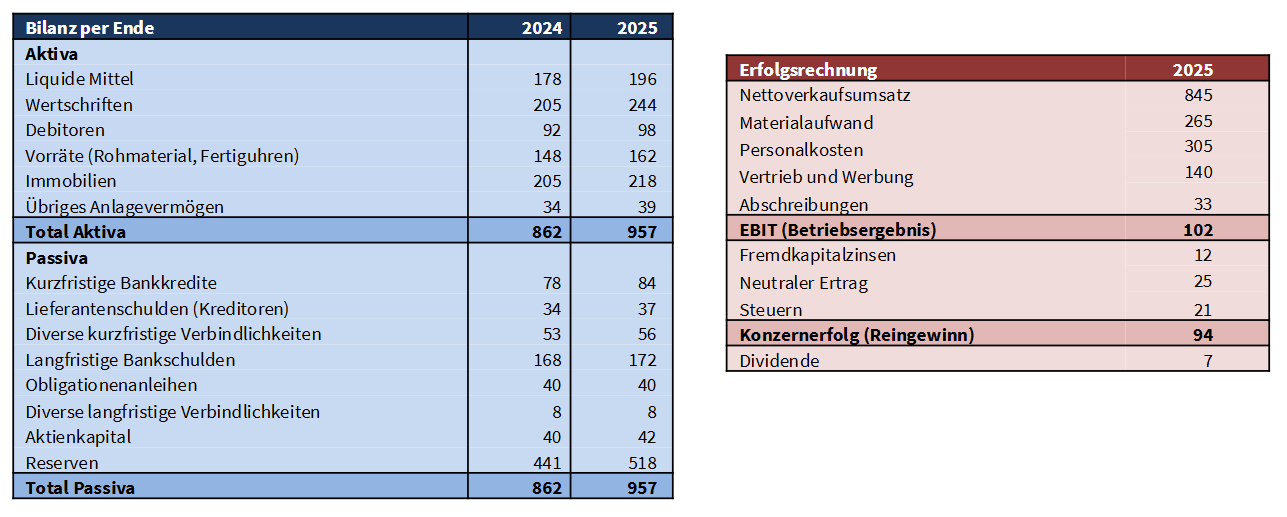
\includegraphics[width=\textwidth,height=0.7\textheight,keepaspectratio]{figures/UebII.png}

\begin{itemize}
    \item Fremdkapital
    \begin{itemize}
        \item Aussenfinanzierung ( Kreditfinanzierung => Bankkredite und Bankschulden +6 + 4 = 10)
        \item Innen (0 CHF Kein Rückstellungskonto)
    \end{itemize}
    \item Eigenkapital
     \begin{itemize}
        \item Aussenfinanzierung (Unterschied Aktienkapital => +2)
        \item Innen
    \end{itemize}
    \item Vermögensverflüssigung
     \begin{itemize}
        \item Aussenfinanzierung 
        \item Innen
    \end{itemize}
\end{itemize}

\subsection{Beteiligungsfinanzierung und Agio}
\begin{itemize}
    \item Kapitalerhöhung mit
    \begin{itemize}
        \item N = Nennwert 
        \item X = Emissionspreis
        \item Agio = Emissionspreis - Nennwert
    \end{itemize}
\end{itemize}
\begin{definition}
    [Agio] ist die ''Belohnung'' des Aktienemittenten oder Vermittlers
\end{definition}

\subsection{Bezugsrecht}

Wenn Aktienkapital Erhöhung geplant, müssen bisherige Aktionäre jeweils Anteil an neue Aktien erhalten um Verwässerung des Werts und Mitstimm/Eigentumsrecht zu schützen.

Berechnet:
\begin{equation}
    S_neu = \cdot \frac{S_alt \cdot a + X * \triangle_neu}{a + n} 
\end{equation}
\begin{equation}
    Bezugsrecht = S_alt - S_neu = \frac{S_alt- X}{\frac{a}{n} + 1}
\end{equation}

\subsection{Leverage Effekt}


